% Page: Markov chains
% prob-06-markov-chains.qmd
% Reflected walk on the non-negative integers. From 0 the chain steps to 1
% with probability p and stays with probability q=1-p. From j>=1 it steps to
% j+1 with probability p and to j-1 with probability q. The balance equations
% give pi_j = (p/q)^j pi_0, which sum to 1 only when p<q, and then
% pi_0 = 1-p/q. The bars are that formula at p/q = 1/2.
\documentclass[border=6pt]{standalone}
\usepackage[T1]{fontenc}
\usepackage{lmodern}
\usepackage{amsmath,amssymb}
\usepackage{tikz}
\usetikzlibrary{arrows.meta}
\usepackage{pgfplots}
\pgfplotsset{compat=1.18}
\definecolor{ink}{HTML}{1F2430}
\definecolor{statblue}{HTML}{174A7E}
\definecolor{bluefill}{HTML}{D7E5F0}
\definecolor{grey}{HTML}{5E6A75}
\pgfplotsset{
  stat/.style={
    scale only axis,
    axis lines=left,
    axis line style={ink, line width=0.6pt},
    tick style={ink, line width=0.45pt},
    tick label style={font=\small, text=ink},
    label style={font=\small, text=ink},
    title style={font=\small, text=ink, align=center},
    unbounded coords=jump,
    scaled ticks=false,
  },
}
\begin{document}
\begin{tabular}{@{}l@{}}
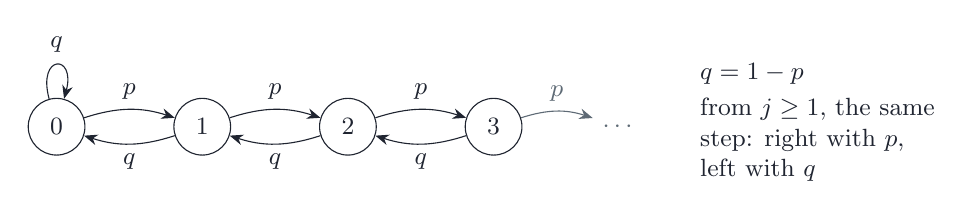
\begin{tikzpicture}[
  font=\small,
  every node/.style={text=ink},
  st/.style={circle, draw=ink, thin, minimum size=7.2mm, inner sep=0pt},
  trans/.style={-{Stealth[length=1.7mm,width=1.35mm]}, ink, thin},
]
  \node[st] (s0) at (0,0) {$0$};
  \node[st] (s1) at (1.85,0) {$1$};
  \node[st] (s2) at (3.70,0) {$2$};
  \node[st] (s3) at (5.55,0) {$3$};
  \node[grey] (dots) at (7.15,0) {$\cdots$};

  \draw[trans] (s0) edge[loop above, looseness=8] node[above=1pt] {$q$} (s0);
  \draw[trans] (s0) to[bend left=18] node[above] {$p$} (s1);
  \draw[trans] (s1) to[bend left=18] node[below] {$q$} (s0);
  \draw[trans] (s1) to[bend left=18] node[above] {$p$} (s2);
  \draw[trans] (s2) to[bend left=18] node[below] {$q$} (s1);
  \draw[trans] (s2) to[bend left=18] node[above] {$p$} (s3);
  \draw[trans] (s3) to[bend left=18] node[below] {$q$} (s2);
  \draw[trans, grey] (s3) to[bend left=18] node[above, text=grey] {$p$} (dots);

  \node[anchor=west, align=left, font=\small] at (8.05,0.05)
    {$q=1-p$\\[2pt]
     from $j\ge 1$, the same\\
     step: right with $p$,\\
     left with $q$};
\end{tikzpicture}
\\[10pt]
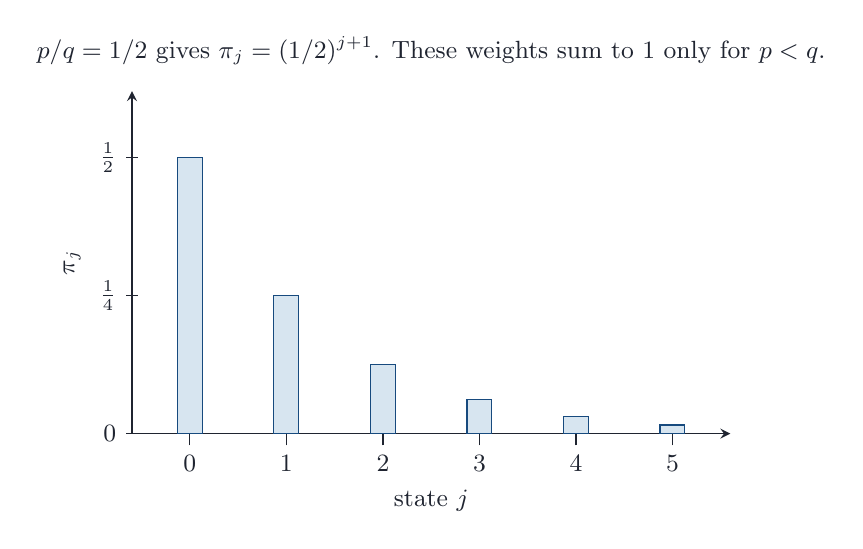
\begin{tikzpicture}
\begin{axis}[
  stat, width=7.6cm, height=4.35cm,
  xmin=-0.6, xmax=5.6, ymin=0, ymax=0.62,
  xtick={0,1,2,3,4,5},
  ytick={0,0.25,0.5},
  yticklabels={$0$,$\tfrac14$,$\tfrac12$},
  xlabel={state $j$},
  ylabel={$\pi_j$},
  title={$p/q=1/2$ gives $\pi_j=(1/2)^{j+1}$. These weights sum to $1$ only for $p<q$.},
  ybar, bar shift=0pt, bar width=9pt,
]
  \addplot[fill=bluefill, draw=statblue, thin, forget plot] coordinates {
    (0,0.5) (1,0.25) (2,0.125) (3,0.0625) (4,0.03125) (5,0.015625)
  };
\end{axis}
\end{tikzpicture}
\end{tabular}
\end{document}
